\documentclass[a4paper,11pt,pdftex]{article}

\usepackage{a4wide}
\usepackage{fancyhdr}
\usepackage{float}
\usepackage[pdftex]{graphicx}
\usepackage[pdftex]{hyperref}

\hypersetup{
        pdftitle   = A PThreads Tracing framework,
        pdfauthor  = Isaac Jurado Peinado,
        pdfsubject = Software instrumentation and tracing,
        colorlinks = true,
        linkcolor  = black,
        citecolor  = black,
        filecolor  = black,
        urlcolor   = blue
}

%\pagestyle{fancy}
%\fancyfoot{}
%\renewcommand{\footrulewidth}{0pt}
%\fancyhead{\thepage}

\setlength{\parindent}{0pt}
\renewcommand{\url}[1]{\href{#1}{#1}}

\newfloat{listing}{H}{lol}[section]
\floatname{listing}{Listing}

\title{A PThreads Tracing framework}
\author{Isaac Jurado Peinado}

\begin{document}

\maketitle
\tableofcontents
\listoffigures
\listof{listing}{List of Code Listings}

\setlength{\parskip}{.7\baselineskip plus .2\baselineskip minus .1\baselineskip}
\newpage

\section{Introduction}

This documents presents PTT\footnote{Which stands for \textbf{P}OSIX
\textbf{T}hreads \textbf{T}racing}: a simple, easy to use and semi automatic
framework for tracing multi-threaded applications that make use of the POSIX
Threads standard API.  The tracing is achieved by means of a manual source code
instrumentation, supported by some automated processes.  Thus, categorizing this
tool as a library would not be completely correct because the build system also
plays an important role in the instrumentation activity.

Section \ref{sec:applications} explains how to instrument an application and
provides an example taken from the PARSEC
benchmarks\footnote{\url{http://parsec.cs.princeton.edu}}.  Section
\ref{sec:framework} describes the overall design of PTT as well as some
important details.  Finally, section \ref{sec:conclusions} discusses the lessons
learned after completing the project.

\section{Instrumenting applications}
\label{sec:applications}

The PTT framework reduces the process of instrumenting an application to three
steps:

\begin{enumerate}
\item Integrate the source into the build system.
\item Define the partial PCF files.
\item Insert the API calls in the code.
\end{enumerate}

This process can be shortened even more, because the second step is optional.
But tu illustrate it completely, the rest of the section is explains the details
with the aid of a real example: the \emph{blackscholes} benchmark, from the
PARSEC suite.

The PTT dependencies for compilation are:

\begin{itemize}
\item GNU make.
\item GNU C compiler and linker.
\item A minimal UNIX environment, including some implementation of AWK
available.
\end{itemize}


\subsection{Build system integration}

The \emph{blackscholes} application consists of one source file, therefore
compiling it is straight forward.  For simplicity, the source is contained in
the directory \verb:parsec: and the tracing library source is reachable by
following the relative path \verb:../ptt/tracelib:.  Then, the first step is to
create a \verb:Makefile:.  The contents are listed in listing
\ref{code:makefile1}.

\begin{listing}
\label{code:makefile1}
\caption{A simple \texttt{Makefile}}
\begin{verbatim}
  PTT_PATH := ../ptt/tracelib
  PROGRAMS := blackscholes
  blackscholes_SOURCES := blackscholes.c
  blackscholes_LIBS := m

  include $(PTT_PATH)/rules.mk
\end{verbatim}
\end{listing}

That is the minimum build rules necessary to generate instrumented binaries.
The first, second and last lines are mandatory, otherwise the build system does
not know what to build nor where to find the tracing library.  It is possible to
have many binaries handled by the same \verb:Makefile:; but for each of the
listed programs, the \verb:program_SOURCES: variable needs to be specified.
Note that header files can also be included in it, and it will provide more
dependency information.  For example, suppose there was another application in
the same directory as the example, the \verb:Makefile: would then look like
listing \ref{code:makefile2}.

\begin{listing}
\label{code:makefile2}
\caption{A \texttt{Makefile} to handle multiple programs}
\begin{verbatim}
  PTT_PATH := ../ptt/tracelib
  PROGRAMS := blackscholes otherprog
  blackscholes_SOURCES := blackscholes.c
  blackscholes_LIBS := m
  otherprog_SOURCES := main.c module.c module.h

  include $(PTT_PATH)/rules.mk
\end{verbatim}
\end{listing}

Also for each program specified in the \verb:PROGRAM: variable, it is possible
to define a \verb:prog_LIBS: and \verb:prog_PCF: variables.  The former is a
list of libraries needed at link time.  In the example, \emph{blackscholes}
needs the math library (\verb:-lm: compiler switch).  Note that it is not
necessary to explicitly specify the linkage against the \emph{PThreads} library,
as it it assumed by the build system.  The latter will be explained later on.

At this stage, it is already possible to compile running just \verb:make:.  It
generates a binary called \verb:blackscholes: which, after each execution,
generates three files named \verb:ptt-trace-000:\footnote{The last numbers are
incremented to preserve already existing files} with extensions ``\verb:.prv:'',
``\verb:.pcf:'' and ``\verb:.row:''.  These are the files needed by Paraver to
visualize a trace.

\begin{figure}
\centering
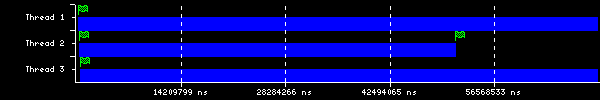
\includegraphics{pics/bs-stage1.png}
\caption{Resulting trace with no manual instrumentation}
\label{fig:bs-stage1}
\end{figure}

So, with no modification in the source code yet, the binary generates traces
containing minimal information about thread creation, destruction and eventual
event flushing operations.  Figure \ref{fig:bs-stage1} shows an example.


\subsection{Event definition}
\label{sec:pcf_sample}

Although this step is optional, it can become very helpful when manipulating
resulting traces.  The purpose is to enhance the human readable event
information provided to Paraver.

The idea is to write directly a \textbf{partial} PCF\footnote{\emph{Paraver
Configuration File}} file, or multiple files.  That is, write event and value
definitions that will be appended to the basic PCF file, provided by the
framework.

In the example, a \emph{Phase} event could be defined, with several possible
values:

\begin{listing}
\label{code:pcf1}
\caption{A simple PCF file}
\begin{verbatim}
  EVENT_TYPE
  0    7000    Phase
  VALUES
  0      None
  1      Running
  2      Mutex wait
  3      Critical section
  4      Barrier wait
\end{verbatim}
\end{listing}

Now it is necessary to acknowledge the existence of this new file to the build
system.  Therefore, listing \ref{code:makefile1} should be changed to what is
shown by listing \ref{code:makefile3} following, assuming that listing
\ref{code:pcf1} is saved as \verb:blackscholes.pcf:.

\begin{listing}
\label{code:makefile3}
\caption{Second step for the simple \texttt{Makefile}}
\begin{verbatim}
  PTT_PATH := ../ptt/tracelib
  PROGRAMS := blackscholes
  blackscholes_SOURCES := blackscholes.c
  blackscholes_LIBS := m
  blackscholes_PCF := blackscholes.pcf

  include $(PTT_PATH)/rules.mk
\end{verbatim}
\end{listing}

The way events are organized in different files is quite flexible.
Nevertheless, in the end all specified PCF files are concatenated and processed
altogether.  In particular, the variable \verb:PCF_FILES: provides a way to
share a PCF file among all the programs controlled under the same
\verb:Makefile: without having to explicitly add it to each \verb:prog_PCF:
variable.  For example, in order to share the PCF described in listing
\ref{code:pcf1} with all the other programs, an example using the
\verb:PCF_FILES: variable is illustrated by listing \ref{code:makefile4}.

\begin{listing}
\label{code:makefile4}
\caption{Multiple program \texttt{Makefile} sharing a PCF file}
\begin{verbatim}
  PTT_PATH := ../ptt/tracelib
  PROGRAMS := blackscholes otherprog
  PCF_FILES := blackscholes.pcf
  blackscholes_SOURCES := blackscholes.c
  blackscholes_LIBS := m
  otherprog_SOURCES := main.c module.c module.h

  include $(PTT_PATH)/rules.mk
\end{verbatim}
\end{listing}

From here, the build system automatically provides as many derived constants as
events and values defined in all specified PCF files.  The names, though, are
mangled a bit by replacing spaces with underscores and transforming all the
letters to uppercase.  For example, the previous PCF listing would provide the
following constants at compilation time:

\begin{itemize}
\item \verb:PHASE:
\item \verb:NONE:
\item \verb:RUNNING:
\item \verb:MUTEX_WAIT:
\item \verb:CRITICAL_SECTION:
\item \verb:BARRIER_WAIT:
\end{itemize}


\subsection{Inserting events}

Finally, it is time to insert the interesting events to investigate after the
executions, directly from Paraver.  There are two functions, already available
from the build system, that generate events:

\begin{verbatim}
  void ptt_event  (int type, int value);
  void ptt_events (int count, int type1, int value1, ...);
\end{verbatim}

In fact, these are the only functions available to the user.  The reason for the
second function to exist is to provide the ability to generate multiple events
with the exact same time value.  Once instrumented, the binary will generate the
proper files to be interpreted by Paraver.

Note that the instrumented binaries can generate traces with a prefix other than
\verb:ptt-trace: in their filenames.  By setting the \verb:PTT_TRACE_NAME:
environment variable, its contents will be used as a trace filename prefix
instead of the default.

% vim:ft=tex:spell

\section{Framework implementation}
\label{sec:framework}

Once presented the mode of operation from the user point of view, it is time to
dip into the details.  As already mentioned in the introduction, the PTT
framework basically consists of two main components:

\begin{itemize}
\item Build system.
\item Tracing library.
\end{itemize}


\subsection{Build system}

To offer a functionality similar to \emph{automake} the build rules make use of
some advanced features from GNU Make.  Dependencies are properly defined so a
change in the tracing library or one of the preprocessing scripts.  However, the
dependency relationships established between the header and source files of the
user's programs are not as fine grained as they could.  A functionality that was
dropped due to the attached complexity increase to the build system.

Most of the magic involved in the automation explained in section
\ref{sec:pcf_sample} is achieved via simple preprocessing scripts that parse all
the PCF contents concatenated in a single stream.  For each program containing
custom PCF definitions, two files are generated:

\begin{itemize}
\item \verb:pcf_program.h:: containing the symbolic constants for the event
types and values.  This file is also included automatically, so no explicit
inclusion is required.
\item \verb:pcf_program.c:: containing the full PCF contents, in the form of a C
string, to be generated for each execution.
\end{itemize}

In case on extra PCF content is attached to the program, the header file is
not generated.

The build system also takes care of building the library in case it is
necessary, issuing the proper compiler and linker flags and embedding the
tracing library into the program binary.  In particular, one linker flag is of
special interest and it is discussed later in this section.


\subsection{Tracing library}

Using some compiler and linker special trickery allows the library to have most
of its code called automatically, freeing the user from that responsibility.
This approach has two main advantages:

\begin{itemize}
\item Eases the instrumentation process.
\item Reduces the troubleshooting scenarios produced by potential human errors,
like, for example, forgetting to insert a concrete initialization or
finalization function.
\end{itemize}

The automation happens at two levels: process and thread.  Each level needs
initialisation and finalisation.  At the process level, the library makes use of
the special GCC function attributes \emph{constructor} and \emph{destructor}.
They instruct the compiler to add a call before the execution of the main
function, and before finishing the process respectively.

At the thread level, detecting thread finalization is easy thanks to the
destructor function that can be associated to a \verb:pthread_key_t:.  This data
type provides \emph{thread local storage} which, at the same time, it is used by
the library to store separate per thread event buffers.  When the thread
finishes, all its defined \emph{thread local storage} keys are released, also
calling their destructor function, if defined.

Detecting thread creation is a different story.  It is important to
automatically intercept thread creation because the library needs to create
tracing structures for the new thread, otherwise the user would have to do it.
In this case some linker aid is necessary.  The idea is to intercept calls to
the \verb:pthread_create: function to be able to alter some of its parameters;
in particular the thread function and its parameter.  Essentially, once
\verb:pthread_create: is intercepted, the process of creating a thread is the
following:

\begin{enumerate}
\item User calls \verb:pthread_create: providing a function.
\item The call is redirected to the tracing library.
\item The tracing library allocates space for the new tracing structures.
\item The tracing library calls the real \verb:pthread_create: providing a
different function, an internal \emph{proxy} function.
\item The system creates the new thread and calls the proxy function.
\item The proxy function initializes the tracing structures.
\item The proxy function finally calls the user function provided initially.
\end{enumerate}

Focusing now on bare function call interception, there are two main approaches
that do not involve modifying the source code:

\begin{itemize}
\item The \verb:LD_PRELOAD: trick.
\item The linker \verb:--wrap: flag.
\end{itemize}

The first one is a run time solution, which has the advantage of not requiring
recompilation of the program.  It has the downside of requiring a slightly
complex environment to make it work.  Besides, the events are inserted in the
source code so recompilation is still necessary.  This leaves the second
solution.

The GNU linker provides a special \verb:--wrap: flag that allows to modify
external symbol resolution between objects.  The \verb:--wrap: switch requires
an argument: the symbol to catch.  When the linker finds an unresolved reference
to the symbol, e.g. \verb:func:, the reference is redirected to the symbol
\verb:__wrap_func: instead.  Then the linker looks for unresolved references to
the symbol \verb:__real_func:, which is redirected to \verb:func:.

Therefore, with a \verb:__wrap_pthread_create: function defined and the proper
command line switches, the linker does the job and the final binary does not
need any special environment nor library available.


\subsection{Post-processing}

To reduce memory consumption, the event buffers have a limited capacity.  When
buffers are filled they need to be flushed to disk to allow more events to enter
the buffer.  Each thread flushes to its own file to avoid locking, so at the end
of the execution there are as many files as threads have been executed.

At this point the traces need to be merged and each event needs to be adjusted a
bit.  In particular, the time of each event needs to be converted to
nanoseconds.  This is where post processing comes into play.

Inspired by the \emph{Cell Superscalar} framework.  Such post processing stage
is performed within the same process, right at the end of the execution.  This
way the post process can be simplified.

To minimize flush overhead, threads dump their buffers in raw binary form.  If
trace merging was separated from generation, byte endianness should be taken
into account as it would open the possibility of trying to post process binary
traces generated in a different architecture.

On the other hand, binary traces can be considered temporary files and created
as such; which raises the chances to be stored in a local or RAM file system.

Finally, some global information can be kept in main memory, saving the post
processor from having to parse it.


\subsection{Framework limitations}

In PTT, the main and only tracing primitive is the event.  There is no
communication nor state primitives as in other tracing tools.  Neither is the
availability of hardware counters nor, obviously, automatic events added with
such information.

Nevertheless, these limitations are in harmony with the main design goals of
simplicity and ease of use.

% vim:ft=tex:spell

\section{Conclusions}
\label{sec:conclusions}

Two of the most important lessons learned while designing and developing the
framework have been that, firstly, finding the balance between flexibility,
simplicity and functionality is much harder than it seems; and, secondly,
choosing the proper combination of event types and values to instrument an
application is also difficult.

The main obstacle in the design has been the nonexistence of file format
documentation from Paraver.  Specially for the PCF definitions, which could have
been much better exploited and led to better results.

On the personal side, this project has constituted a reminder for the need of
better time management policies and schedules.  But it has been fun so far.

% vim:ft=tex:spell


\end{document}

% vim:ft=tex
